\documentclass[12pt]{article} 
\usepackage[utf8]{inputenc}
\usepackage{geometry}
\geometry{letterpaper}
\usepackage{graphicx} 
\usepackage{parskip}
\usepackage{booktabs}
\usepackage{array} 
\usepackage{paralist} 
\usepackage{verbatim}
\usepackage{subfig}
\usepackage{fancyhdr}
\usepackage{sectsty}

\pagestyle{fancy}
\renewcommand{\headrulewidth}{0pt} 
\lhead{}\chead{}\rhead{}
\lfoot{}\cfoot{\thepage}\rfoot{}

%%% SECTION TITLE APPEARANCE
\allsectionsfont{\sffamily\mdseries\upshape} 

%%% ToC (table of contents) APPEARANCE
\usepackage[nottoc,notlof,notlot]{tocbibind} 
\usepackage[titles,subfigure]{tocloft}
\renewcommand{\cftsecfont}{\rmfamily\mdseries\upshape}
\renewcommand{\cftsecpagefont}{\rmfamily\mdseries\upshape} %

\usepackage{amsmath}
\usepackage{amssymb}

\title{APMA 0350: Homework 8}
\author{Milan Capoor}
\date{11 November 2022}

\begin{document}
\maketitle

\textbf{Problem 1:} Consider the following COVID model with only two types of people S (susceptible) and I (infected) and the following interactions.
\begin{itemize}
    \item S to I: $\frac{b}{N}(I)$
    \item I to S: $\gamma$
    \item N = S + I
\end{itemize}

\begin{enumerate}
    \item Set up a system of ODE for S and I
    
    Solution:
    \[\boxed{\begin{cases}
        S'(t) = \gamma I(t) -\left(\frac{b}{N}\right) S(t)\; I(t) \\
        I'(t) = \left(\frac{b}{N}\right) S(t)\; I(t) - \gamma I(t)
    \end{cases}}\]

    \item Let $\tau = \gamma t$ and 
    \[x(\tau) = \frac{S(\frac{\tau}{\gamma})}{N} \implies S(t) = N x(\gamma t)\]
    \[y(\tau) = \frac{I(\frac{\tau}{\gamma})}{N} \implies I(t) = N y(\gamma t)\]
    \[R_0 = \frac{b}{\gamma}\]

    Rewrite your system in terms of $x$, $y$, $R_0$

    Solution:
    \[\begin{cases}
        S'(t) = \gamma I(t) -\left(\frac{b}{N}\right) S(t) = N \gamma y(\gamma t) - \frac{b}{N} N x(\gamma t) \\
        I'(t) = \left(\frac{b}{N}\right) S(t)\; I(t) - \gamma I(t) = \left(\frac{b}{N}\right) N x(\gamma t)\; N y (\gamma t) - \gamma N y(\gamma t)
    \end{cases}\]
    \[\begin{cases}
        S' = N\gamma x'(\tau) = \gamma Ny(\tau) -\left(\frac{b}{N}\right) Nx(\tau)\; Ny(\tau) \\
        I' = N\gamma y'(\tau) = \left(\frac{b}{N}\right) Nx(\tau)\; Ny(\tau) - \gamma Ny(\tau)
    \end{cases}\]
    \[\begin{cases}
        \gamma x' = \gamma y - bxy\\
        \gamma y' = bxy - \gamma y
    \end{cases}\]
    \[\boxed{\begin{cases}
        x' = y - R_0 xy\\
        y' = R_0 xy - y
    \end{cases}}\]

    \item Find the equilibrium points in the system in (b) as well as their
    stability
    \[\begin{cases}
        x' = 0 = y(1 - R_0 x)\\
        y' = 0 = y(R_0 x - 1)
    \end{cases}\]
    So, 
    $y= 0$ or $x = 1/R_0$ 
    and the equilibria are 
    $(x, 0)$ and $(\frac{1}{R_0}, y)$

    \[\nabla F(x, y) = \begin{bmatrix}
        \frac{\partial x'}{\partial x} & \frac{\partial x'}{\partial y}\\
        \frac{\partial y'}{\partial x} & \frac{\partial y'}{\partial y}
    \end{bmatrix} = \begin{bmatrix}
        -R_0 y & 1 - R_0 x\\
        R_0 y & R_0x - 1
    \end{bmatrix}\]

    \[\nabla F(x, 0) = \begin{bmatrix}
        0 & 1 - R_0 x\\
        0 & R_0 x - 1
    \end{bmatrix}\]
    Eigenvalues: $\lambda = 0$ and
    \[\lambda = R_0 x - 1 = \begin{cases}
       \lambda < 0 \quad \text{ for }\, x < \frac{1}{R_0}\\
        \lambda > 0 \quad \text{ for }\, x > \frac{1}{R_0}
    \end{cases}\]
    \boxed{\text{So solutions of the form (x, 0) are stable when $x < \frac{1}{R_0}$}}

    \[\nabla F(1/R_0, y) = \begin{bmatrix}
        -R_0 y & 0\\
        R_0 y & 0
    \end{bmatrix}\]
    Eigenvalues: $\lambda = 0$ and $\lambda = -R_0 y$ 
    \[\lambda = -R_0 y = \begin{cases}
        \lambda < 0 \quad \text{ for }\, y > 0\\
        \lambda > 0 \quad \text{ for }\, y < 0
    \end{cases}\]
    \boxed{\text{So solutions of the form $(1/R_0, y)$ are stable when $y > 0$}}

    \item In the case $R_0 < 1$, draw a phase portrait similar to what was done in lecture (no need to study the x = 0 axis). What happens to the solutions in the long-run? Will the disease die out in this case?
    \[R_0 < 1 \implies 1 < 1/R_0\]
    \[x \leq 1 \implies x < 1/R_0 \]
    So all solutions of the form $(x, 0)$ are stable

    Similarly, because $0 \leq y \leq 1$, solutions of the form $(1/R_0, y)$ are also stable. 

    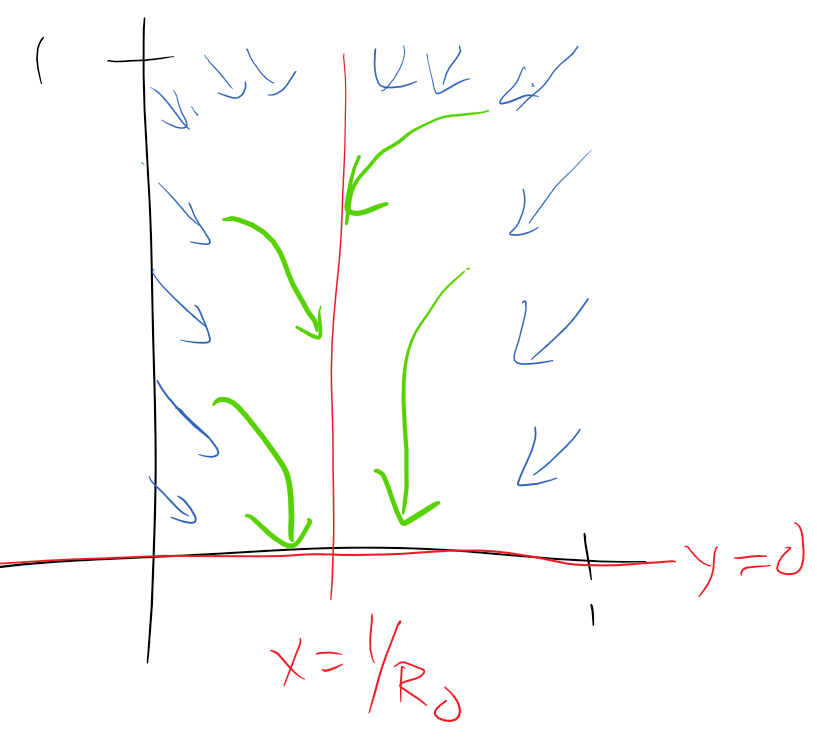
\includegraphics{Images/SI equilibria 1.png}

    In this case, solutions will eventually go to zero \boxed{\text{so the disease will die out}}. 

    \item In the case $R_0 > 1$, draw a phase portrait with your equilibria and their stability, as well as solutions that start with $x > 1/R_0$ (don't worry what happens if $x < 1/R_0$). Will the disease die out
    in this case?
    \[R_0 > 1 \implies 1/R_0 < 1\]
    So solutions on $y = 0$ will be stable when $x < \frac{1}{R_0}$ and unstable above that. 

    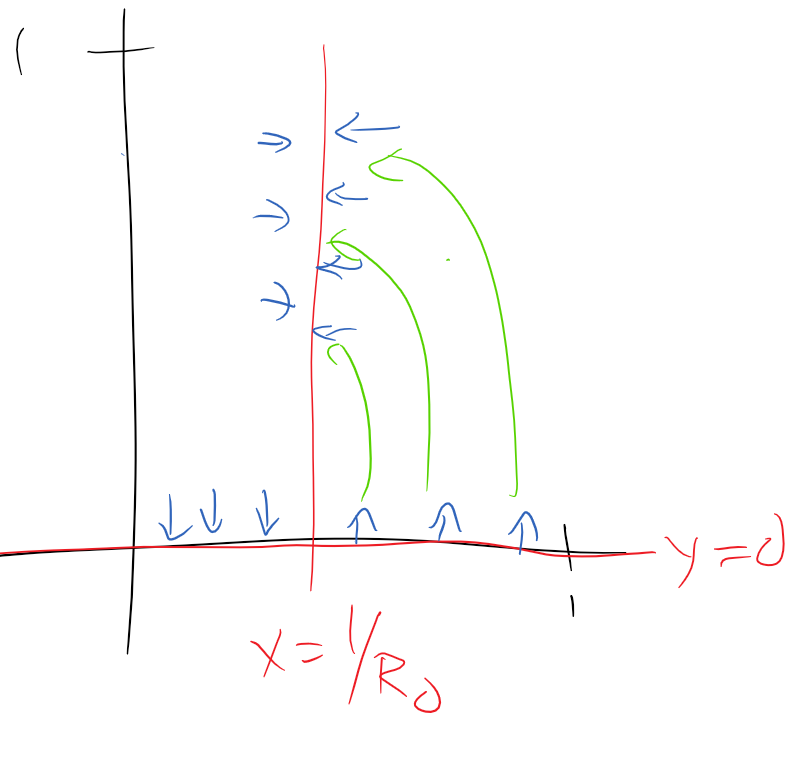
\includegraphics{Images/SI equilibria 2.png}

    In this case, because the 0 solutions is unstable and people can be reinfected, \boxed{\text{the pandemic will continue forever}}
\end{enumerate}

\pagebreak 

\textbf{Problem 2:} You work as a consultant for PeyAlamo, a car rental company that has distributors in Atlanta and Boston. Travelers may rent a car in one city and return it either at the same location or the other city. The company wants to determine how to distribute their cars optimally among the two cities. They provide you with the following data: 40\% of the cars rented in Atlanta are returned in Boston per day, and 20\% of cars rented in Boston are returned in Atlanta per day. Let x(t) and y(t) be the number of cars in Atlanta and Boston respectively, where t is in days.

\begin{enumerate}
    \item Set up an ODE 
    \[\begin{cases}
        x'(t) = 0.2y(t) - 0.4x(t)\\
        y'(t) = 0.4x(t) - 0.2y(t)\\
    \end{cases}\]

    \item Find the equilibrium points and classify 
    \[\begin{cases}
        x' = 0 = 0.2 (y - 2x)\\
        y' = 0 = 0.2 (2x - y)
    \end{cases} \implies y = 2x\]
    \[\nabla F(x, y) = \begin{bmatrix}
        \frac{\partial x'}{\partial x} & \frac{\partial x'}{\partial y}\\
        \frac{\partial y'}{\partial x} & \frac{\partial y'}{\partial y}
    \end{bmatrix} = \begin{bmatrix}
        -0.4 & 0.2\\
        0.4 & -0.2
    \end{bmatrix}\]
    \[\nabla F(x, 2x) = \begin{bmatrix}
        -0.4 & 0.2\\
        0.4 & -0.2
    \end{bmatrix}\]
    Eigenvalues:
    \[(-0.4 - \lambda)(-0.2 - \lambda) - 0.08 = 0\]
    \[0.6\lambda + \lambda^2 = \lambda(\lambda + 0.6) = 0\]
    \[\lambda = \{0, \; -0.6\}\]
    \boxed{\text{So the solutions of the form $(x, 2x)$ are stable }}

    \pagebreak 

    \item Draw a phase portrait that includes your equilibrium points and 4 solutions on each side of your equilibria. 
    
    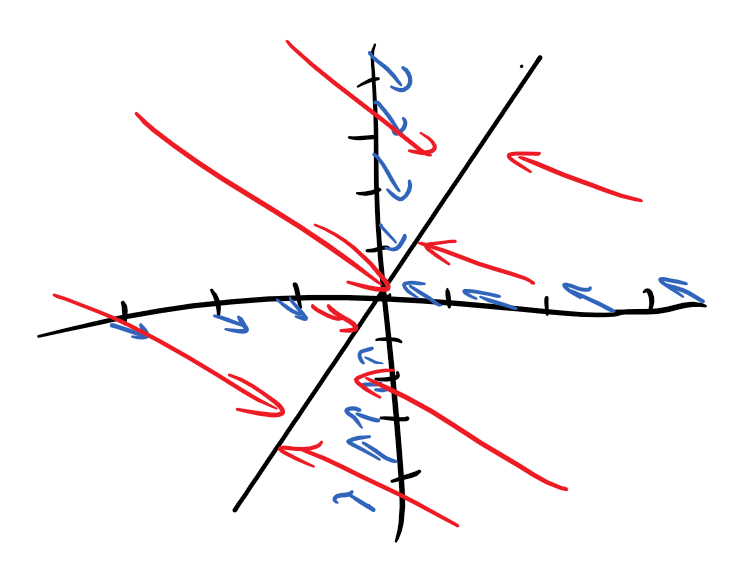
\includegraphics{Images/p2 solutions.png}

    \item What happens to the solutions $(x(t), y(t))$ in the long-run? In particular, what can you tell me about the ratio $y(t)/x(t)$ ?
    
    All solutions are drawn to the stable line of equilibrium $y = 2x$ so in the long run,
    \[\lim_{t \to \infty} \frac{y(t)}{x(t)} = \frac{2x}{x} = \boxed{2}\]
    
    \item If you were the CEO of PeyAlamo and your company owned 1200 cars, how many parking spots would you rent in Atlanta and how many in Boston?
    \[x + y = 1200\]
    \[x + 2x = 1200 \implies x = 400, \; y = 800\]
    \boxed{\text{So I would place 400 cars in Atlanta and 800 in Boston}}
\end{enumerate}

\pagebreak 

\textbf{Problem 3:} Find the general solution of the following ODE
\begin{enumerate}
    \item $y'' = y' + y$
    Solution:
    \[r^2 - r - 1 = 0\]
    \[r = \frac{1 \pm \sqrt{1 - 4(-1)}}{2} = \frac{1 \pm \sqrt{5}}{2} = \pm \phi\]
    \[\boxed{y = Ae^{\phi t} + B e^{-\phi t}}\]

    \item $6y'' - 7y' + 2y = 0$
    Solution:
    \[5r^2 - 7r  +2 = 0\]
    \[(5r - 2)(r - 1) = 0 \implies r = \{1, \; \frac{2}{5}\}\]
    \[\boxed{y = Ae^{t} + Be^{2t/5}}\]
    
    \item An ODE with auxiliary equation $(r - 1)r(r + 1)(r+ 2) = 0$
    Solution:
    \[\boxed{y = A + Be^t + Ce^{-t} + De^{-2t}}\]
\end{enumerate}

\pagebreak 

\textbf{Problem 4:} Solve the following ODE
\[\begin{cases}
    y'' - 3y' - 28y = 0\\
    y(0) = 3\\
    y'(0) = 1
\end{cases}\]

Solution:
\[r^2 - 3r - 28 = 0\]
\[r = \frac{3 \pm \sqrt{9 - 4(-28)}}{2} = \frac{3 \pm 11}{2} \implies r = \{7, \; -2\}\]  
\[y = Ae^{7t} + Be^{-2t}\]
\[\begin{cases}
    y(0) = A + B = 3\\
    y'(0) = 7A - 2B = -1
\end{cases} \implies \begin{cases}
    7(3 - B) - 2B = -1 \implies 21 - 9B = -1 \implies B = 22/9\\
    A + \frac{22}{9} = 3 \implies A = \frac{5}{9}
\end{cases}\]

\[\boxed{y = \frac{5}{9}e^{7t} + \frac{22}{9}e^{-2t}}\]
\end{document}